\chapter{Estruturas de um Sistema RAV}
Os conceitos e definições necessárias para o desenvolvimento deste trabalho, foram apresentados nos capítulos anteriores, neste capítulo será apresentando toda a estrutura para implementação do sistema de reconhecimento de voz.

O sistema RAV proposto, foi implementado para um sistema independente do locutor, visando um jogo divertido para o maior número de pessoas possíveis, com o modo de pronúncia de palavras isoladas, e um vocabulário pequeno, que faz parte de um diciónario pré-definido. 

Este sistema foi desenvolvido em Java, com suas Apis e direcionada para sistemas operacionais Android, tendo como base a teoria dos Modelos Ocultos de Markov para o modelamento de sequencias de frames. Então cada elocução é dividida em quadros de tempos com iguais durações, extraindo seus parâmetros de cada um deles para se criar os modelos Hmms para cada palavra do dicionário, como sistemas de reconhecimento de palavras isoladas necessitam da captura do início e fim das palavras pronunciadas, o usuário deve pronunciar um comando, e depois de um breve intervalo, pronunciar o próximo, os comandos disponíveis no dicionário da aplicação são: “Direita”, “Esquerda”, “Acima” e “Abaixo”. O personagem do jogo só responderá ao comando dito, depois de reconhecer qual é o comando falado, em caso de sucesso, o jogo continua normalmente, até a vitória ou derrota do jogador, em caso do não reconhecimento da palavra, o sistema ignora a palavra dita. Outra característica importante do reconhecedor é a tentativa de capturar o humor do jogador com palavras ofensivas gravadas no dicionário, o sistema apresenta uma penalidade em caso dessas palavras serem pronunciadas.

Este trabalho pode ser dividido em 6 etapas: Aquisição da fala, Pré-Processamento, Extração de Parâmetros, Criação de referências, Classificação e Execução dos comandos.

\section{Aplicação RAV}
\begin{figure}[H]
\includegraphics[width=0.8\textwidth]{graficos/desenvolvimento_rav.eps}
\caption{Diagrama de Atividades do Sistema}
\end{figure}

Com resultado da transcrição, são definidos os comandos do jogo.

\section{Aquisição da fala}

A interação do usuário com a aplicação é feita apenas com a voz, ao iniciar o sistema, a interface de voz com usuário é habilitada, permitindo ao usuário interagir com os comandos definidos no vocabulário. Como a aplicação é destinada a dispositivos móveis, a captura do som, é feita pelo microfone do celular ou tablet, fornecendo um sinal elétrico, sendo nessário uma filtragem do sinal analógico resultante por um filtro passa-baixas, chamado de anti-aliasing, para depois ser feita a conversão analógio-digital \cite{DigitalProcRabiner}. Esse filtro tem o intuito de suprimir componentes de frequência superiores à metade da frequência de amostragem, sendo chamado de Nyquist \cite{DigitalSigProakis}.

A última etapa da aquisição da fala é a conversão do sinal de fala analógico em digital através de um
amostrador, possibilitando o processamento digital. Segundo \citeonline{PattRecChou} é nesta fase que são
escolhidas a taxa de amostragem, impossibilitando a ocorrência do efeito de aliasing e a precisão usada para a gravação do sinal, a partir do número de níveis que esse sinal poderá assumir. 
Todas etapas podem ser vistas na subseção \ref{subsec:fala} deste trabalho.


\section{Pré-Processamento}
Sistemas RAV sofrem com características do ambiente de gravação e o canal de comunicação, como ruídos de alta frequência, distância do microfone, períodos de silêncio, etc. Uma forma de amenizar esse proplemas é fazer o sinal passar por um processo chamado de pré-processamento, deixando o sinal mais próximo da fala pura. As etapas desse processo podem ser mostradas na figura 7 \cite{RavIsolAnderson}. 

\begin{figure}[H]
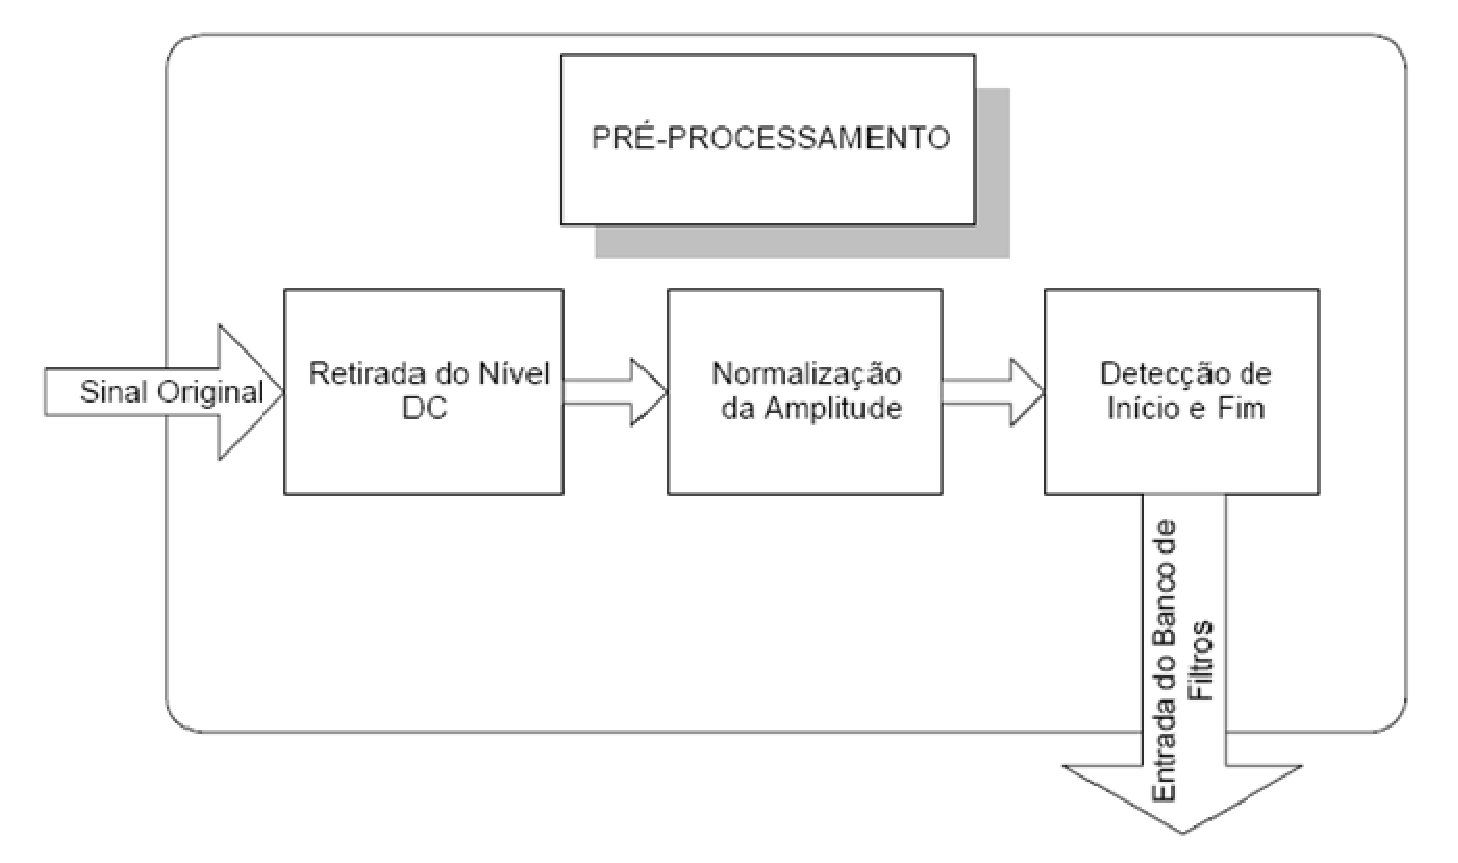
\includegraphics[width=0.8\textwidth]{graficos/pre_proc.eps}
\caption{Diagrama de blocos da fase de pré-processamento}
\end{figure}

Calculando a média aritmétrica das amplitudes do sinal digital e subtraindo de cada aplitude esta média, consegue-se retirar o nível DC, que é uma componente contínua que atrapalha a comparação em valores absolutos. Outro problema encontrado é o diferencial entre sons mais baixos e sons mais altos, que é resolvido com a normalização da amplitude, esse pré-processamento do sinal faz com que todos os valores de amplitude de todos os sinais estejam na faixa de -1 e 1, garantindo que esses sinais sejam processados igualmente no algoritmo de reconhecimento. Esse processo é possível dividindo o valor de cada amostra do sinal pelo maior valor de aplitude do mesmo. 

A última fase do pré-processamento no sistema RAV de palavras isoladas é a detecção do início e fim da locução, a fim de remover de forma precisa períodos de silêncio, que podem conter ruídos, sinais indesejados e a duração do sinal falado \cite{RavIsolAnderson}. De acordo com \citeonline{SpeechCodChu} esse processo também tem como objetivo diminuir a carga computacional e economizar tempo, já que o sistema poderá processar apenas trechos que fazem parte da fala.
 O extremo inicial é determinado pelo primeiro quadro onde realmente se inicia a fala e o extremo final é
determinado pelo último quadro que ainda há fala.

\section{Extração de Parâmetros} 
A extração de parâmetros é uma etapa de grande importância em um sistema RAV, pois o sinal digital possui uma grande quantidade de dados e uma análise direta necessitaria tempo e processamento consideráveis e ainda sim, não apresentariam um resultado expressivo. 


\section{Treinamento dos Modelos Ocultos de Markov}
A fase de treinamento é uma das etapas de maior importancia em um sistema de reconhecimento de voz independente do locutor e ser o fator determinante na obtenção de um sistema com bons resultados ou não. É o momento em que são definidos os modelos HMMs para cada palavra do vocabulário utilizado.

A definição da quantidade de estados necessários para modelar uma palavra e o número de misturas por estado não são definidos por uma regra, mas sim, dependente da familiaridade com os modelos HMMs ou por intuição, além de serem necessários muitos testes para obtenção do melhor resultado. 
%Escrever a quantidade de estados e misturas no momento da implentação

%\subsection{Aquisição do sinal de voz}


%\subsection{Pré-Processamento} 


 





